\documentclass[10pt]{article}

\usepackage{amsmath}

\newcommand{\myvec}[1]{\ensuremath{\begin{pmatrix}#1\end{pmatrix}}}

\newcommand{\mydet}[1]{\ensuremath{\begin{vmatrix}#1\end{vmatrix}}}

\newcommand{\solution}{\noindent \textbf{Solution: }}

\providecommand{\brak}[1]{\ensuremath{\left(#1\right)}}

\providecommand{\norm}[1]{\left\lVert#1\right\rVert}
\usepackage{graphicx}
\usepackage{float}

\let\vec\mathbf
\title{Coordinate-Geomentry}
\author{Paidisetty Rithik(paidisettyrithik@sriprakashschools.com)}

\begin{document}
\maketitle
\section*{10$^{th}$ Maths - Chapter 7}
This is Problem-8 from Exercise 7.2
\begin{enumerate}
\item if $\vec{A}$ and $\vec{B}$ are\myvec{-2\\-2} and \myvec{2\\-4},respectively,find the coordinates of $\vec{P}$ such that $\vec{AP}$=$\frac{3}{7}\vec{AB}$ and $\vec{P}$ lies on the segment $\vec{AB}$ \\
\end{enumerate}
\solution \\
Given,\\
$\vec{A}$=\myvec{-2\\-2}, $\vec{B}$=\myvec{2\\-4},
$m_1:m_2=3:4$
\begin{align}
\vec{P}=\frac{m_1B+m_2A}{m_1+m_2}\\
\vec{P}=\frac{3\myvec{2\\-4}+4\myvec{-2\\-2}}{3+4}\\
\vec{P}=\frac{\myvec{6-8\\-12-8}}{3+4}\\
\vec{P}=\myvec{\frac{6-8}{3+4}\\\frac{-12-8}{3+4}}\\
\vec{P}=\myvec{\frac{-2}{7}\\\frac{-20}{7}}
\end{align}

\begin{figure}[H]
			\centering
			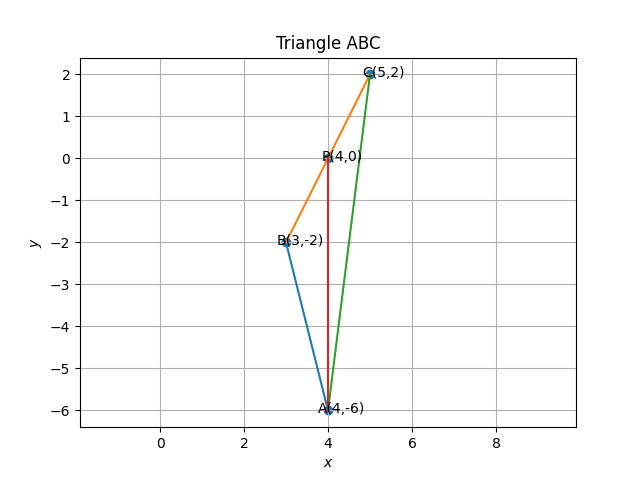
\includegraphics[width=\columnwidth]{figs/Figure_1.png}
			\caption{Line segment AB}
			\label{fig:4}
		\end{figure}


\end{document}
